\documentclass[conference]{IEEEtran}
\usepackage[T1]{fontenc}
\usepackage{graphicx,booktabs,amsmath,cite,url}
\usepackage[hidelinks]{hyperref}
\usepackage{xcolor}

\begin{document}

\title{The Token Tax on Indian Languages: Measuring Tokenizer Premiums Across All 22 Scheduled Languages and 14 Tokenizers}

\author{\IEEEauthorblockN{<<AUTHOR>>}
\IEEEauthorblockA{Independent Researcher<<EMAIL_LINE>>}}

\maketitle

\begin{abstract}
Large language models (LLMs) process text as subword tokens, and the number of tokens a text requires determines API cost, usable context length and generation latency. Tokenizers built from English-dominated data segment other languages into more tokens, imposing a ``token tax''. We measure this tax for all 22 scheduled languages of India using 1,024 professionally translated parallel sentences (IN22-Gen) and 14 tokenizers, including GPT-4o, Llama~4, Gemma~3, DeepSeek-V3, Qwen~3 and the Indian-built Sarvam-1, Krutrim-2, IndicBERT~v2 and MuRIL. Relative to English, GPT-4o needs <<gpt4o_mean>>$\times$ as many tokens on average (<<gpt4o_hi>>$\times$ for Hindi, <<gpt4o_worst>>$\times$ for Santali), and the most efficient LLM tokenizer, Gemma~3, needs <<gemma_mean>>$\times$. Newer tokenizers roughly halve the premium of their predecessors, but not for the scripts with the least web presence. Sarvam-1 is the most efficient LLM tokenizer on its ten target languages (<<sarvam10>>$\times$) yet less efficient than GPT-4o on the remaining twelve. Using human romanizations from the Dakshina dataset, we find that romanized input is cheaper only for older, English-centric tokenizers and costs <<r_indic_range>> more on Indic-focused ones. Finally, Unicode NFC normalization changes token counts by between $-$<<nfc_sarvam_bn>>\% and +<<nfc_mbert_bn>>\% depending on the tokenizer. We also document a library-level discrepancy that inflated GPT-4o counts by about 46\% and describe the verification protocol that caught it. Code and data are released.
\end{abstract}

\begin{IEEEkeywords}
tokenization, multilingual NLP, Indian languages, large language models, fairness, romanization
\end{IEEEkeywords}

\section{Introduction}
Subword tokenizers based on byte-pair encoding or unigram language models~\cite{sennrich2016,kudo2018} map text to the units an LLM reads and generates. Because most commercial APIs bill per token, and context windows and decoding time are also counted in tokens, a language that needs more tokens to express the same content is more expensive, fits less text into context and is slower to generate. Prior work has shown that this ``tokenization premium'' varies widely across the world's languages~\cite{petrov2023,ahia2023}.

India has 22 languages listed in the Eighth Schedule of its Constitution, written in at least 13 scripts. Several are spoken by tens of millions of people, while others, such as Santali (Ol Chiki script) and Manipuri (Meitei Mayek script), have a very small web footprint. Recent tokenizers have greatly expanded their vocabularies, and several Indian organizations have released models designed for Indian languages. This raises a practical question: \emph{how large is the token tax on Indian languages today, and who pays the most?}

This paper makes four contributions:
\begin{enumerate}
\item A measurement of the token premium for all 22 scheduled languages on a professionally translated parallel corpus, across 14 current tokenizers, including four Indian-built ones (Section~\ref{sec:results}).
\item A verification protocol for token counting, which revealed that loading a community conversion of GPT-4o's tokenizer through a popular library over-counted tokens by about 46\% (Section~\ref{sec:verify}).
\item An analysis of romanized versus native-script input on human-written romanizations (Section~\ref{sec:roman}).
\item A measurement of how Unicode normalization changes token counts (Section~\ref{sec:nfc}).
\end{enumerate}

\section{Related Work}
Petrov et al.~\cite{petrov2023} defined the tokenization premium on parallel FLORES-200 sentences and showed premiums above 10$\times$ for some languages. Ahia et al.~\cite{ahia2023} analyzed the resulting cost and utility disparities for commercial APIs. Rust et al.~\cite{rust2021} linked tokenizer quality to downstream monolingual performance. For Indian languages, MuRIL~\cite{khanuja2021} and IndicBERT~v2~\cite{doddapaneni2023} built encoder vocabularies specifically for Indic scripts. IN22~\cite{gala2023} provides professionally translated evaluation data for all 22 scheduled languages, and Dakshina~\cite{roark2020} provides human romanizations for South Asian languages. We extend this line of work with current LLM tokenizers, full coverage of the 22 scheduled languages, Indian-built LLM tokenizers, and the romanization and normalization questions.

\section{Data and Method}
\subsection{Corpora}
\textbf{IN22-Gen}~\cite{gala2023}: 1,024 general-domain English sentences, each professionally translated into all 22 scheduled languages. Because every language expresses the same content, token counts are directly comparable. We use the openly downloadable MTEB copy of the test split.
\textbf{Dakshina}~\cite{roark2020}: Wikipedia sentences in native script paired with human-written romanizations. We use the 11 Indian languages it covers (about 10,000 sentence pairs each, empty rows removed).

\subsection{Tokenizers}
Table~\ref{tab:tok} lists the 14 tokenizers: ten used by LLMs and four by encoder models. Krutrim-2's tokenizer has exactly the same vocabulary as Mistral NeMo's (identical counts on every sentence; Krutrim-2 is built on Mistral NeMo~\cite{krutrim2,mistralnemo}), so the two are reported as one. GPT-4o and GPT-4 are counted with OpenAI's official \texttt{tiktoken}~\cite{tiktoken}. All other tokenizers are loaded from their \texttt{tokenizer.json} file with the Hugging Face \texttt{tokenizers} library, except MuRIL (WordPiece vocabulary only), which uses \texttt{transformers}. Special tokens are never added.

\subsection{Metrics}
For tokenizer $t$ and language $\ell$, with $n_t(\ell)$ the total number of tokens for the 1,024 sentences, the \emph{token premium} is
\begin{equation}
\pi_t(\ell) = n_t(\ell)\, /\, n_t(\text{English}).
\end{equation}
A premium of 1 means parity with English. We also report \emph{fertility} (tokens per whitespace-separated word). Encoder vocabularies map unseen characters to a single \texttt{[UNK]} token, which makes a text look cheap only because it is discarded. We therefore exclude a $(t,\ell)$ cell when more than 2\% of its tokens are \texttt{[UNK]}; this removes 7 languages for mBERT, 3 for XLM-R and 2 for MuRIL. We also record the share of byte-fallback tokens (\texttt{<0xNN>}), which signals characters missing from the vocabulary. Confidence intervals are 95\% paired bootstrap intervals over sentences (1,000 resamples)~\cite{efron1993}.

\subsection{Verification}\label{sec:verify}
In our first run, GPT-4o's counts were far higher than expected. On a 3,450-sentence check set, the community \texttt{tokenizer.json} conversion of GPT-4o's tokenizer produced 466,327 tokens when loaded through \texttt{transformers} (v5.22.1), but 319,957 when loaded directly with \texttt{tokenizers}, which matched OpenAI's \texttt{tiktoken} exactly on all 3,450 sentences. The same discrepancy was 4\% for GPT-4. For every other tokenizer, both loading paths gave identical counts. A warning recommending a regex fix flag changed nothing for Mistral NeMo and wrongly altered counts for BERT-style tokenizers, so it was not used. We recommend verifying token counts against an official implementation before reporting them.

\begin{table*}[t]
\caption{Tokenizers and mean token premium over the 22 scheduled languages, with 95\% bootstrap CI and the cheapest and most expensive language. $^*$Excludes languages with $>$2\% \texttt{[UNK]} tokens (mBERT 7, XLM-R 3, MuRIL 2).}
\label{tab:tok}
\centering\footnotesize\setlength{\tabcolsep}{5pt}
\begin{tabular}{@{}llrcll@{}}
\toprule
Tokenizer & Developer & Vocab. & Mean premium [95\% CI] & Cheapest language & Most expensive language \\
\midrule
\multicolumn{6}{@{}l}{\emph{LLM tokenizers}} \\
<<TABLE_LLM>>
\midrule
\multicolumn{6}{@{}l}{\emph{Encoder tokenizers}} \\
<<TABLE_ENC>>
\bottomrule
\end{tabular}
\end{table*}

\section{Results}\label{sec:results}
\subsection{Overall premium}
Among LLM tokenizers, the mean premium ranges from <<gemma_mean>>$\times$ (Gemma~3) to <<gpt4_mean>>$\times$ (GPT-4) (Table~\ref{tab:tok}). GPT-4o, the tokenizer behind many deployed applications, averages <<gpt4o_mean>>$\times$. For an application billed per token, the same content therefore costs roughly three times as much in the average Indian language as in English, and a fixed context window holds roughly a third as much text. The bootstrap intervals are narrow (about $\pm$0.05), so the differences between tokenizers are not sampling noise. The Indic-focused encoder vocabularies reach <<indicbert_mean>>$\times$ (IndicBERT~v2) and <<muril_mean>>$\times$ (MuRIL), which shows that near-parity is achievable: the tax is a design choice rather than a property of the languages.

\begin{figure*}[t]
\centering
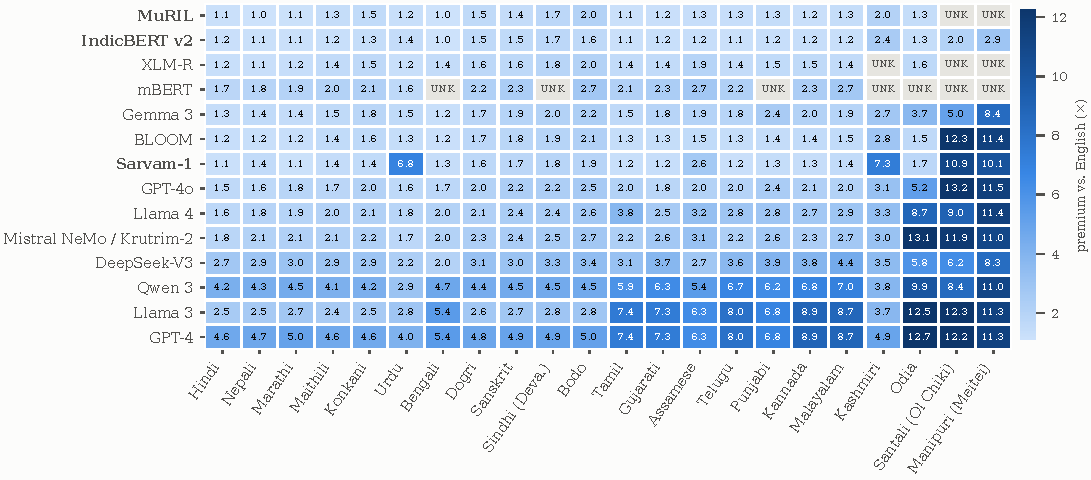
\includegraphics[width=\textwidth]{figs/fig1_heatmap.pdf}
\caption{Token premium relative to English for each tokenizer and language (IN22-Gen). Rows are sorted by mean premium and columns by mean premium across tokenizers. Bold labels mark Indian-built tokenizers. UNK: cell excluded because more than 2\% of tokens are \texttt{[UNK]}.}
\label{fig:heat}
\end{figure*}

\subsection{Variation across languages}
The language matters more than the tokenizer (Fig.~\ref{fig:heat}). Averaged over tokenizers, the cheapest languages are Hindi (<<avg_hindi>>$\times$), Nepali (<<avg_nepali>>$\times$) and Marathi (<<avg_marathi>>$\times$), all written in Devanagari. The most expensive are Odia (<<avg_odia>>$\times$), Santali in Ol Chiki (<<avg_santali>>$\times$) and Manipuri in Meitei Mayek (<<avg_manipuri>>$\times$). For the last two, most tokenizers fall back to byte-level tokens, spending several tokens per character. Odia illustrates the effect of vocabulary design: <<odia_gpt4o>>$\times$ with GPT-4o, but <<odia_mistral>>$\times$ with Mistral NeMo.

\subsection{Generational change}
Replacing GPT-4's tokenizer with GPT-4o's reduced the mean premium from <<gpt4_mean>>$\times$ to <<gpt4o_mean>>$\times$ (<<gpt_drop>>\% lower), and Llama~3 to Llama~4 from <<llama3_mean>>$\times$ to <<llama4_mean>>$\times$ (<<llama_drop>>\% lower). Fig.~\ref{fig:gpt} shows that the gains are uneven: Telugu fell from <<telugu_gpt4>>$\times$ to <<telugu_gpt4o>>$\times$, but Santali (<<santali_gpt4>>$\times\rightarrow$<<santali_gpt4o>>$\times$) and Manipuri (<<manipuri_gpt4>>$\times\rightarrow$<<manipuri_gpt4o>>$\times$) became slightly more expensive.

\begin{figure}[t]
\centering
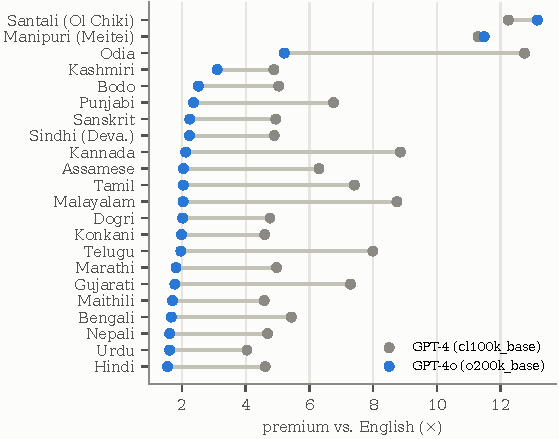
\includegraphics[width=\columnwidth]{figs/fig2_gpt4_vs_gpt4o.pdf}
\caption{Premium per language for GPT-4 (cl100k\_base) and GPT-4o (o200k\_base).}
\label{fig:gpt}
\end{figure}

\subsection{Indian-built tokenizers}
Sarvam-1 targets ten languages (Bengali, Gujarati, Hindi, Kannada, Malayalam, Marathi, Odia, Punjabi, Tamil, Telugu)~\cite{sarvam1}. On these it is the most efficient LLM tokenizer we tested, at <<sarvam10>>$\times$ versus <<gemma10>>$\times$ for Gemma~3 and <<gpt4o_10>>$\times$ for GPT-4o (Fig.~\ref{fig:sarvam}). On the other twelve scheduled languages its premium rises to <<sarvam_other>>$\times$, above GPT-4o's <<gpt4o_other>>$\times$. Perso-Arabic script (Urdu, Kashmiri) falls back almost entirely to bytes. Sarvam reports a fertility of 1.4--2.1 on its target languages~\cite{sarvam1}. On IN22-Gen we measure <<sarvam_fert_min>>--<<sarvam_fert_max>>, with <<sarvam_fert_in_range>> of the ten languages inside the reported range. The difference may reflect text domain or word segmentation, but it shows that efficiency claims depend on the evaluation text. Krutrim-2 inherits Mistral NeMo's premium (<<mistral_mean>>$\times$ on average).

\begin{figure}[t]
\centering
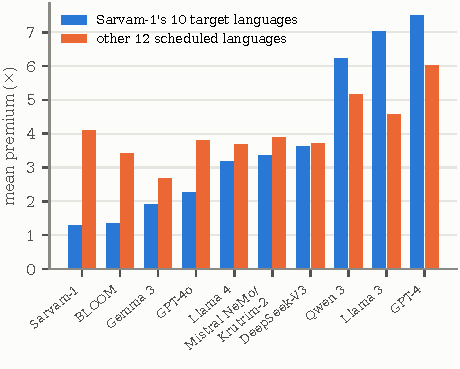
\includegraphics[width=\columnwidth]{figs/fig3_sarvam_split.pdf}
\caption{Mean premium of LLM tokenizers on Sarvam-1's ten target languages versus the other twelve scheduled languages.}
\label{fig:sarvam}
\end{figure}

\subsection{Romanized versus native script}\label{sec:roman}
Many users type Indian languages in Latin script. Fig.~\ref{fig:roman} compares token counts for the same Dakshina sentences in human romanization and native script. For English-centric tokenizers, romanization is much cheaper: <<r_gpt4_pct>>\% fewer tokens with GPT-4, <<r_llama3_pct>>\% with Llama~3 and <<r_qwen_pct>>\% with Qwen~3. For GPT-4o the two are nearly equal (ratio <<r_gpt4o>>). For Indic-focused tokenizers romanization is more expensive: <<r_sarvam>>$\times$ for Sarvam-1, <<r_muril>>$\times$ for MuRIL and <<r_indicbert>>$\times$ for IndicBERT~v2. Sarvam-1's low ratios for Urdu and Sindhi arise because these Dakshina languages use Perso-Arabic script, which its vocabulary does not cover. Advice to romanize in order to save tokens is therefore outdated for modern and Indic-focused models.

\begin{figure}[t]
\centering
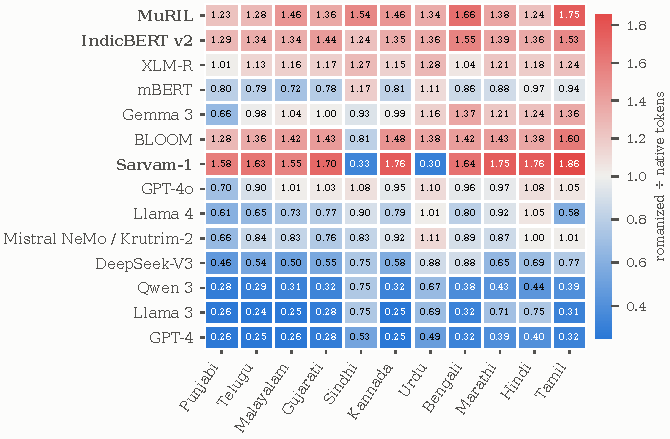
\includegraphics[width=\columnwidth]{figs/fig4_romanized.pdf}
\caption{Ratio of tokens for human-romanized to native-script text (Dakshina). Values below 1 (blue) mean romanized text is cheaper.}
\label{fig:roman}
\end{figure}

\subsection{Unicode normalization}\label{sec:nfc}
Some Indic characters have two canonically equivalent encodings, for example the Bengali letters \emph{yya} and \emph{rra} as single code points or as a base letter plus nukta. Unicode Normalization Form C (NFC)~\cite{uax15} changes 86\% of IN22-Gen's Bengali sentences and 70\% of its Punjabi sentences. Sarvam-1's vocabulary contains only the decomposed forms, so 95\% of its byte fallbacks in Bengali come from these two letters. Table~\ref{tab:nfc} shows that NFC normalization reduces Sarvam-1's Bengali token count by <<nfc_sarvam_bn>>\%, but increases mBERT's by <<nfc_mbert_bn>>\%. Normalization should match the form a tokenizer was trained on, and both forms should be measured.

\begin{table}[t]
\caption{Token count change after NFC normalization (largest effects).}
\label{tab:nfc}
\centering\footnotesize
\begin{tabular}{@{}llr@{}}
\toprule
Tokenizer & Language & Change \\
\midrule
<<TABLE_NFC>>
\bottomrule
\end{tabular}
\end{table}

\section{Discussion and Limitations}
For developers serving Indian users, tokenizer choice is a first-order cost decision. Gemma~3 and GPT-4o are the most efficient general-purpose LLM tokenizers here, and Sarvam-1 is the most efficient within its ten languages. Even with the most efficient tokenizers, budgets should assume 2--4$\times$ the tokens of an English product, and far more for Odia, Santali or Manipuri. For Indian model builders, the encoder results show that near-parity is achievable, and extending coverage to all 22 scheduled languages remains the main gap.

Token counts measure cost and context use, not how well a model understands a language. IN22-Gen is formal general-domain text, and conversational, code-mixed or social-media text may tokenize differently. Dakshina romanizations follow Wikipedia-style sentences, while casual romanization varies widely. Premiums are relative to each tokenizer's own English count, so absolute costs also depend on English efficiency and on per-token prices. Several tokenizers were loaded from public mirrors of the official files.

\section{Conclusion}
The token tax on Indian languages is large but uneven. Current LLM tokenizers charge the average scheduled language between <<gemma_mean>>$\times$ (Gemma~3) and <<qwen_mean>>$\times$ (Qwen~3) the tokens of English, newer tokenizers roughly halve older premiums, and the scripts with the least web presence remain an order of magnitude more expensive. Indian-built tokenizers excel within their target languages but do not yet cover all 22. Practical levers exist, including tokenizer choice, script choice and Unicode normalization, but their effect depends on the tokenizer and must be measured.

\section*{Data Availability}
Code, token counts and figures are available <<REPO_URL>>.

\section*{Acknowledgment}
The author used Claude (Anthropic), an AI assistant, to help write the analysis code, run the measurements and draft this manuscript. The author is responsible for the content of the paper.

\bibliographystyle{IEEEtran}
\bibliography{refs}

\end{document}
